\subsection{Солнечные и лунные затмения. Сарос}
\subsubsection{Полное солнечное затмение}
Диаметр тени спутника при полном центральном затмении (когда центры трёх тел лежат на одной прямой), с большой точностью равен:
\begin{equation}d_\text{т}=2\frac{R_\text{л}(a-R_\text{з})-R_\text{с}(a-R_\text{з})}{a-a_\text{л}}
\end{equation}
Где $R_\text{л}$ --- радиус Луны, $R_\text{з}$ --- радиус Земли, $R_\text{с}$ --- радиус Солнца, $a$ --- расстояние от Земли до Солнца, $a_\text{л}$ --- расстояние от Земли до Луны.

Среднее значение  этой величины около 200 км, максимальное около 215 км. При нецентральном затмении максимальный диаметр тени Луны на поверхности Земли может достигать 270 км (Рис.8).

\begin{figure}[h!]
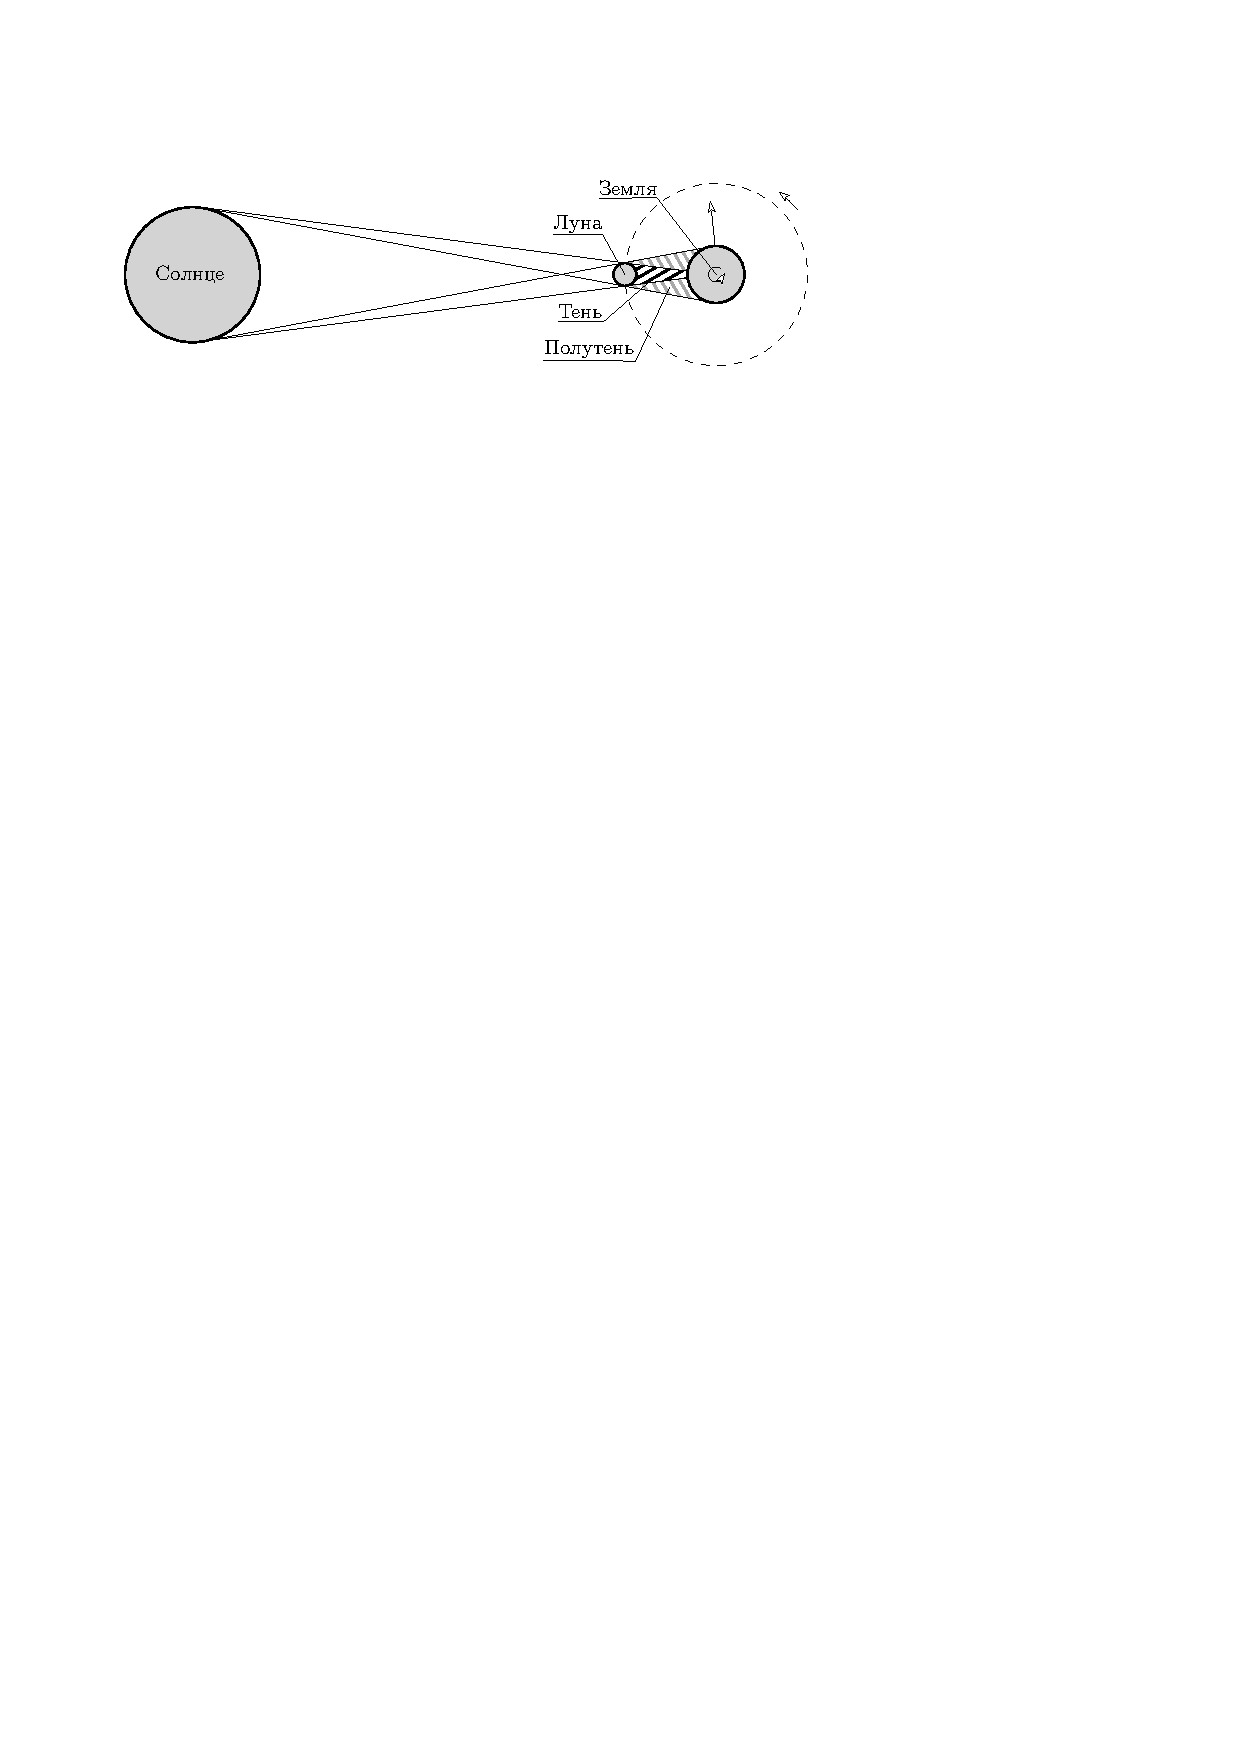
\includegraphics[width = 1.05\textwidth]{full_eclipse}
\caption{Полное солнечное затмение}
\end{figure}

\subsubsection{Кольцеобразное солнечное затмение}
При кольцеобразном солнечном затмении Луна относительно Земли расположена так, что конус её тени не достаёт до поверхности планеты, и вокруг Луны можно наблюдать яркое кольцо незакрытой части солнечного диска (Рис.9).
\begin{center}
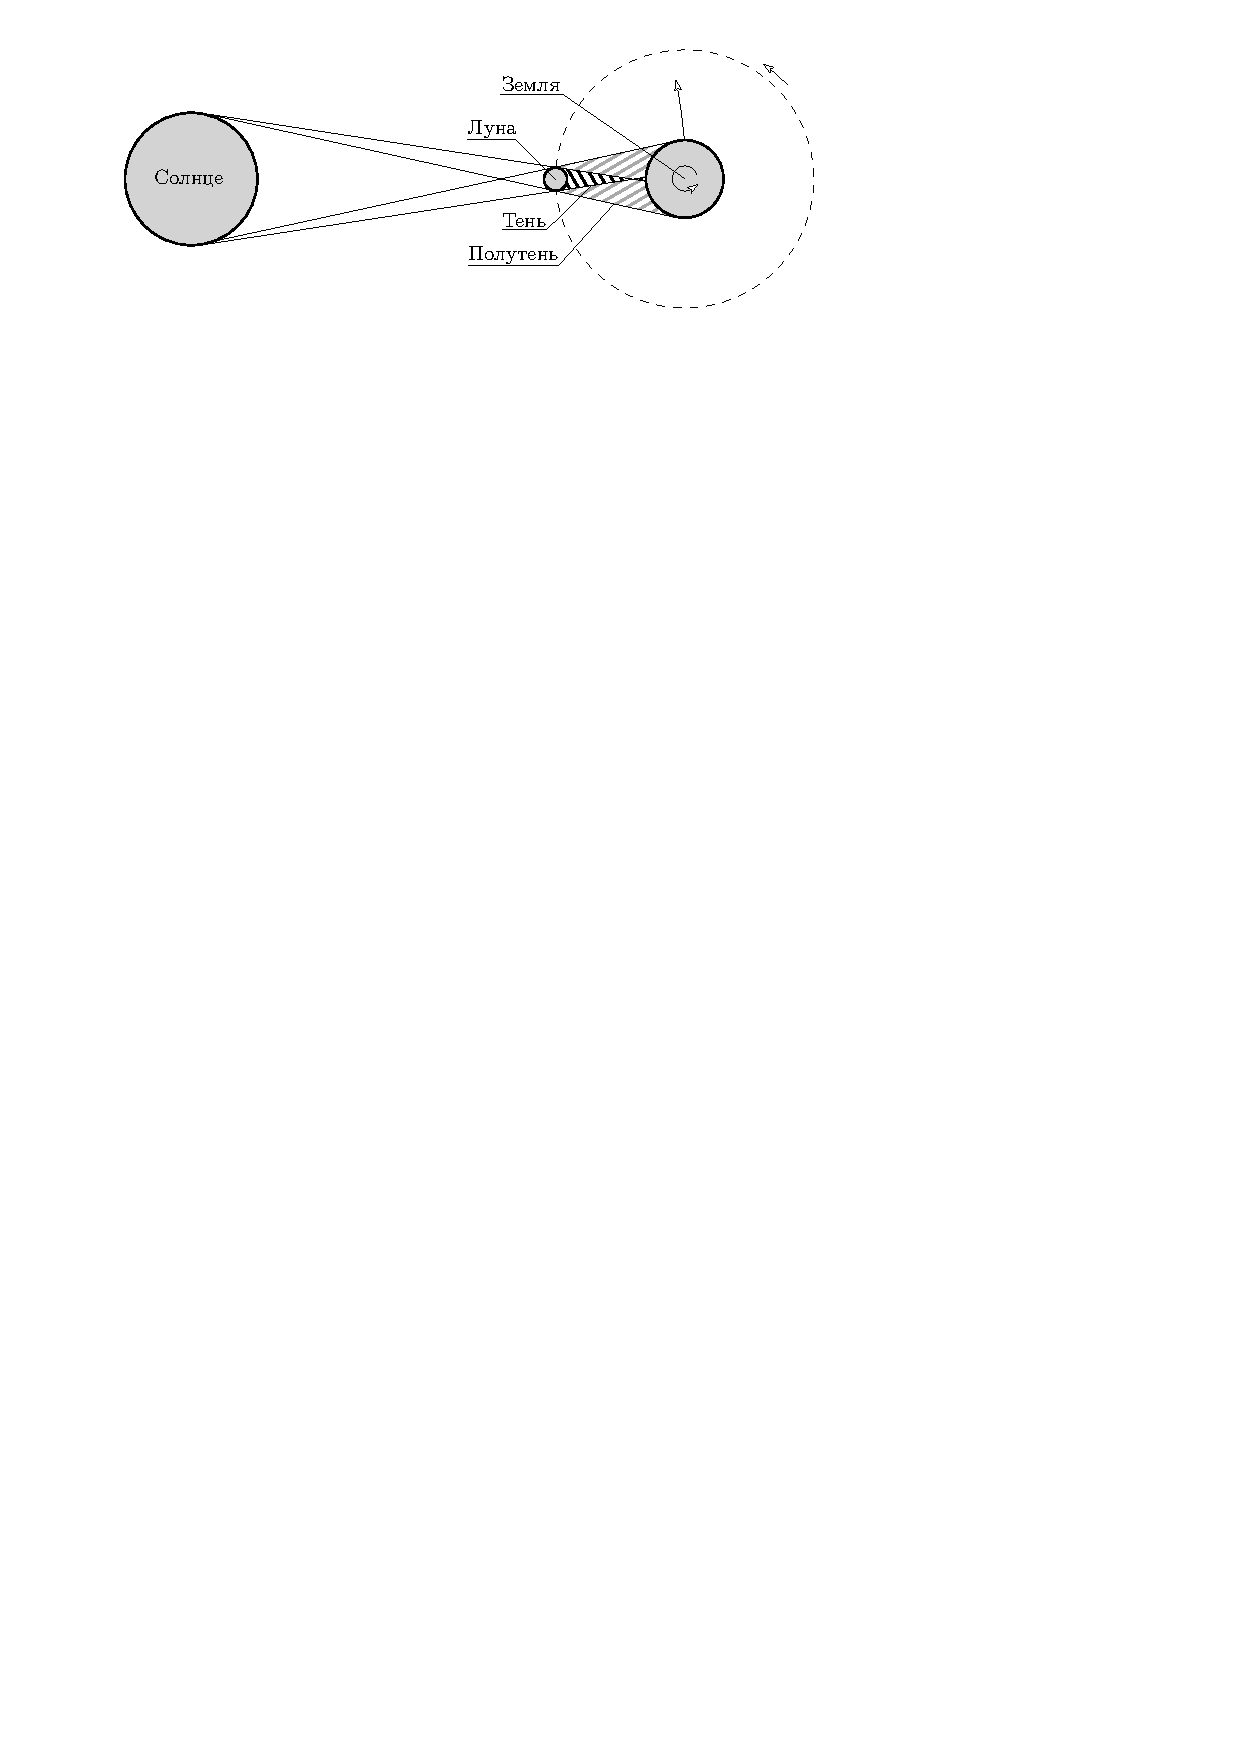
\includegraphics[width = 0.95\textwidth]{partly-eclipse}
\begin{figure}[h!]
\caption{Кольцеобразное солнечное затмение}
\end{figure}
\end{center}
\subsubsection{Лунное затмение}

Лунное затмение в отличие от солнечного, видно со всего ночного полушария. Диаметр земной тени на расстоянии Луны превышает размер последней примерно в 2.5-3 раза (Рис.10).

\textbf{Сарос} --- промежуток  времени, по прошествии которого солнечные и лунные затмения повторяются в прежнем порядке.

Этот период почти в точности равен:
\begin{enumerate}
\item 242 драконических месяца;
\item 223 синодических месяца;
\end{enumerate}

Таким образом, сарос длится примерно 18 лет 11 дней 8 часов.

\textbf{Синодический месяц} --- промежуток времени между одинаковыми фазами Луны. Он равен 29.53 суток.

\textbf{Драконический месяц} --- промежуток времени между двумя последовательными прохождениями Луны через один и тот же узел орбиты. Драконический месяц равен 27.21 суток.
\begin{center}
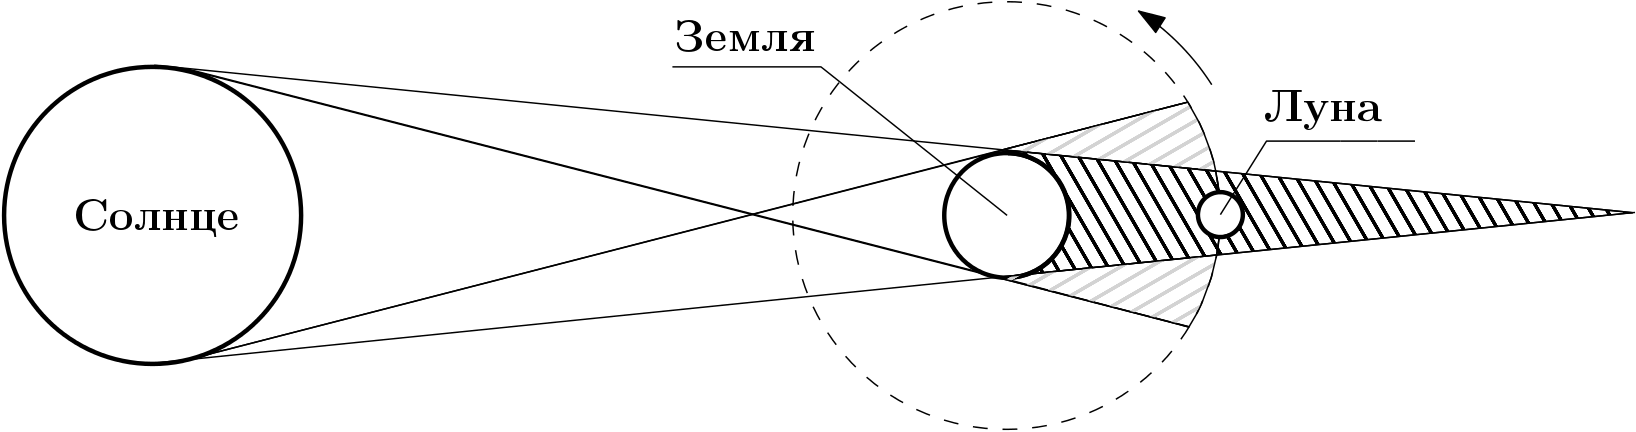
\includegraphics[scale=0.27]{moon-eclipse}
\begin{figure}[h!]
\caption{Лунное затмение}
\end{figure}
\end{center}
\subsubsection{Фаза затмения}
Очень важной характеристикой любого затмения является его фаза. \textbf{Фаза затмения} --- отношение закрытой части диаметра затмеваемого тела, проходящей через уентр затмевающего тела, к полному диаметру затмеваемого тела. Для полного затмения эта величина считается немного иначе (см. ниже). Для Луны затмевающим "телом" является тень Земли. Фазу частного и полного затмения можно вычислить по слейдующим формулам (Рис.11):
\begin{equation}\Phi_{\text{ч}}=\frac{x}{D}
\end{equation} \text{ и } \begin{equation}\Phi_{\text{п}}=1+\frac{d}{D}
\end{equation}
Где $D$ --- диаметр затмеваемого тела.
\begin{center}
\includegraphics[width = 0.3\textwidth]{phases}
\includegraphics[width = 0.3\textwidth]{phases-2}
\begin{figure}[h!]
\caption{Частное и полное затмение}
\end{figure}
\end{center}

Иногда вводят такое понятие, как \textbf{площадная фаза затмения}, т.е. отношение площади закрытой части диска затмеваемого диска к полоной площади его диска. Чаще площадную фазу используют применительно к двойным звёздам, когда считают падение блеска при затмении одной звезды другой.